% !TeX spellcheck = en_US
\documentclass[french]{yLectureNote}

\title{Mécanique}
\subtitle{Mécanique du point}
\author{Paulhenry Saux}
\date{\today}
\yLanguage{Français}

\professor{S.Deheuvels}%sebastien.deveuhels.irap.omp.eu

\usepackage{graphicx}%----pour mettre des images
\usepackage[utf8]{inputenc}%---encodage
\usepackage{geometry}%---pour modifier les tailles et mettre a4paper
%\usepackage{awesomebox}%---pour les boites d'exercices, de pbq et de croquis ---d\'esactiv\'e pour les TP de PC
\usepackage{tikz}%---pour deiffner + d\'ependance de chemfig
\usepackage{tkz-tab}
\usepackage{chemfig}%---pour deiffner formules chimiques
\usepackage{chemformula}%---pour les formules chimiques en \'equation : \ch{...}
\usepackage{tabularx}%---pour dimensionner automatiquement les tableaux avec variable X
\usepackage{awesomebox}%---Pour les boites info, danger et autres
\usepackage{menukeys}%---Pour deiffner les touches de Calculatrice
\usepackage{fancyhdr}%---pour les en-t\^ete personnalis\'ees
\usepackage{blindtext}%---pour les liens
\usepackage{hyperref}%---pour les liens (\`a mettre en dernier)
\usepackage{caption}%---pour la francisation de la l\'egende table vers Tableau
\usepackage{pifont}
\usepackage{array}%---pour les tableaux
\usepackage{lipsum}
\usepackage{yFlatTable}
\usepackage{multicol}
\newcommand{\Lim}[1]{\lim\limits_{\substack{#1}}\:}
\renewcommand{\vec}{\overrightarrow}
\newcommand{\norm}[1]{||\vec{#1}||}
\DeclareMathOperator\arctanh{arctanh}
\begin{document}

%\titleOne
\setcounter{chapter}{2}
	\chapter{Systèmes du premier ordre }
Dans ce chapitre, on va considérer des forces du type $\vec{F_f} = -\alpha\vec{v}$ avec $\alpha$ une constante positive.

\section{Mouvement avec frottements fluides}
\subsection{Exemple : Largage d'un colis}
\subsubsection{Travail préparatoire}
\begin{multicols}{2}
\includegraphics[scale=0.5]{carton}
\columnbreak

Système  = Colis M. On se met dans le référentiel terrestre muni du repère $R$

On fait un bilan des forces : $\vec{P}, \vec{F_f} = -\alpha\vec{v}$

On écrit le PDF : $m\vec{a} = \sum \vec{F}$

Donc  $m\vec{a} = \vec{P}+ \vec{F_f}$

\end{multicols}

On projette les forces : $\vec{P} = -mg\vec{e_y}$ et
$\vec{F_f} = -\alpha(V_x\vec{e_x}+V_y\vec{e_y})$\marginCritical{Lorsque l'on projette la force, on ne sait rien du vecteur vitesse, on ne peut pas formellement savoir sa direction (m\^eme si on peut s'en douter), c'est pourquoi le signe de $\vec{F_f}$ est indépendant de l'axe choisi.}

On réécrit le PFD, projeté selon les axes :
\[
 \left\{\begin{matrix}
 m\ddot{x} =& 0 + -\alpha\dot{x}\\
 m\ddot{y} =& -mg + -\alpha\dot{y}
\end{matrix}\right.
\]
\newpage
\subsubsection{On transforme les équations}

\begin{multicols}{2}
On obtient une équation linéaire :

\[
 \left\{\begin{matrix}
 m\dot{v_x} =& 0 + -\alpha v_x\\
 m\dot{v_y} =& -mg + -\alpha v_y
\end{matrix}\right.
\]

On l'écrit sous la forme canonique

\[
 \left\{\begin{matrix}
 m\dot{v_x} + \alpha v_x =& 0\\
 m\dot{v_y} +\alpha v_y =& -mg
\end{matrix}\right.
\]
\setlength{\columnseprule}{0.4pt}
On divise tout par $m$ :

\[
 \left\{\begin{matrix}
\dot{v_x} +\frac{\alpha}{m} v_x =& 0\\
 \dot{v_y} +\frac{\alpha}{m} v_y =& -g
\end{matrix}\right.
\]
On pose $\tau  = \frac{m}{\alpha}$ :

\[\left\{\begin{matrix}
\dot{v_x} +\frac{1}{\tau} v_x =& 0\\
 \dot{v_y} +\frac{1}{\tau} v_y =& -g
\end{matrix}\right.
\]
\end{multicols}


\subsubsection{On résout les équations}
\paragraph{Première équation}
Elle est homogène, donc de la forme $v_x(t) = Ce^{-t/\tau}$.

À $t=0, v_x(0) = Ce^0 = C$, donc $C = V_0$\marginTips{On se sert des conditions initiales pour déterminer $C$}. Donc $v_x(t) = V_0e^{-t/\tau}$\marginInfo{$v_x(t)\rightarrow 0$ quand $x\rightarrow+\infty$. Au fil du temps, la vitesse horizontale faiblie.}.
\paragraph{Seconde équation}
Elle est non homogène : On écrit donc l'équation sous forme homogène : $\dot{v}_{y,h}(t) + \frac{1}{\tau} v_{y,h} = 0$. Donc : $v_{y,h} = De^{-t/\tau}$.

On cherche ensuite une solution particulière. Le second membre est constant, on cherche $v_{y,p}$ constant, (avec sa dérivée nulle). On obtient $0 + \frac{v_{y,p}}{\tau} = -g \iff v_{y,p} = -\tau g$.

Donc, $v_y(t) = De^{-t/\tau} - \tau g$\marginCritical{On trouve la valeur de D à partir de la solution complète, et non à partir de la solution homogène.}.

À $t=0, v_y(0)=0$. Donc $v_y(0) = De^0-\tau g = D-\tau g = 0 \iff D = \tau g$.

Finalement, en faisant la somme de solution générale et particulière, on trouve : $v_y(t) = \tau g(e^{-t\tau}-1)$.

On va tendre vers un vecteur vitesse $v_{lim} = 0\vec{e_x} -\tau g \vec{e_y} = -\tau g \vec{e_y}$\marginTips{La vitesse tend vers une constante, l’accélération est nulle.}

\subsubsection{Intégration}
\paragraph{Première équation}
On intègre $v_x(t)$ : $x(t) = -\tau V_0e^{-t/\tau} + A$.

Avec les conditions initiales : $x(t=0) = 0$, donc $x(t=0) = -\tau V_0+A = 0 $ et $A = \tau v_0$. $x(t)$ tend vers $\tau V_0$ quand $x$ tend vers l'infini.
\paragraph{Seconde équation}
On intègre $v_y(t)$ : $y(t) = \tau g(-\tau e^{-t/\tau}-t) + B = \tau^2ge^{-t/\tau}-\tau g t + B$. Avec les conditions initiales : $y(0) = h$ et $y(t=0) = \tau^2ge^{-t/\tau}-\tau g t + B$ et $B = h + \tau^2g$.
\subsubsection{Détermination de la durée nécéssaire pour que $v_y$ atteigne 95\% du régime établi}

$v_y$ tend vers $-\tau g$, vitesse limite. On veut $v_y(t_{95}) =0.95\times -\tau g$. Donc $\tau g e^{-t_{95}/\tau} = 0.05\tau g$, donc $t_{95} = -\tau \ln(0.05)$. Donc au bout de $3\tau$, $v_y$ atteint 95\% de sa valeur limite.\marginTips{Si le temps de chute est petit devant $\tau$, on calcule la tangente à $v_y$ au voisinage de 0 en calculant la dérivée de $v_y$, qui est l'accélération. L'équation de la tangente en 0 est $-gt$.}
\section{Radioactivité}
\subsection{Types de réactions}
\warningInfo{Types de Radioactivité}{
Radioactivité $\alpha$ : $^A_ZX\rightarrow _{Z-2}^{A-4}X' + ^4_2\alpha + \gamma$

Radioactivité $\beta +$ : $^A_ZX\rightarrow _{Z-1}^{A}X' + ^0_1e + \nu + \gamma$ avec $\nu$ un neutrino.

Radioactivité $\beta -$ : $^A_ZX\rightarrow _{Z+1}^{A}X' + ^0_{-1}e + \bar{\nu} + \gamma$ avec $\bar{\nu}$ un antineutrino.}


Capture électronique : $^A_ZX + ^0_{-1}e \rightarrow _{Z-1}^{A}X' + \nu + \gamma + X$ avec $X$ des rayons $X$
\subsection{Lois de décroissance radioactive}
Pour chaque réaction radioactive, on peut déterminer la probabilité de désintégration du noyau pendant un intervalle de temps compris entre $t$ et $t+dt$.

On alors $dP = \lambda dt$. Dans le SI, $\lambda$ est en $s^{-1}$.\marginInfo{Si $\lambda$ est donné en $s^{-1}$, si il est donné en année$^{-1}$, T est en années.}

Si on dispose de $n$ noyaux, on peut déterminer le nombre de désintégrations par seconde = $N\times \lambda dt$.

Donc la variation du nombre de noyaux $n$ pendant $dt$ : $dN = -N\lambda dt$. On divise tout par $dt$ : $\frac{dN}{dt} = -\lambda N$, et on aboutit à une EQD du premier ordre linéaire à coefficients constants : $\frac{dN}{dt} +\lambda N= 0 $

On cherche une solution du type $Ce^{rt}$ avec $r=-\lambda$, donc $N(t) = Ce^{-\lambda t}$. Si à $t=0$, $N(0) = N_0$ noyaux, alors $C=N_0$ et $N(t) = N_0e^{-\lambda t}$.

Période de demie-vie $T$ : temps au bout duquel le nombre initial de noyaux est divisé par $2$ :\marginCritical{Pour déterminer la durée de vie moyenne de l'échantillon $\tau$, on fait $\tau = \frac{1}{\lambda}$. Tout comme pour la vitesse limite, au bout de 3$\tau$, on aura fait disparaître 95\% de l'échantillon, il en restera donc plus que 5\%.}\marginTips{Pour réduire au milliéme l'échantillon, il faut 10 $T$ car  $\frac{ \frac{\ln(1000)}{\lambda} }{ \frac{\ln(2)}{\lambda} } = \frac{\ln(1000)}{\ln(2)} \simeq \frac{\ln(2^{10})}{\ln(2)} = 10 \frac{\ln(2)}{\ln(2)} = 10$}

\begin{flalign*}
N_0e^{-\lambda t} &= \frac{N_0}{2}\\
e^{-\lambda t} &= \frac{1}{2}\\
\ln(e^{-\lambda t}) &= \ln(\frac{1}{2})\\
-\lambda T &= -\ln(2)\\
T &= \frac{\ln(2)}{\lambda}
\end{flalign*}


\subsection{Activité}
Définition : Nombre de désintégrations par seconde. Elle se mesure en Becquerel (Bq). \[A(t) = \lambda \times N(t) =  \lambda N_0e^{-\lambda t}\]
\subsection{Élément fils}
$M(t) = $ nombre de noyaux de l'élément fils, soit le nombre d'éléments père détruits. \[M(t) = N_0-N(t) = N_0(1-e^{-\lambda t})\]



\end{document}

